\documentclass{article}
\usepackage[utf8]{inputenc}
\usepackage[T1]{fontenc} % Use 8-bit encoding that has 256 glyphs
\usepackage{fourier} % Use the Adobe Utopia font for the document - comment this line to return to the LaTeX default
\usepackage[english]{babel} % English language/hyphenation
\usepackage{amsmath,amsfonts,amsthm} % Math packages
\usepackage{changepage}
\usepackage{graphicx}
\usepackage{sectsty} % Allows customizing section commands
\allsectionsfont{\centering \normalfont\scshape} % Make all sections centered, the default font and small caps

\usepackage{fancyhdr} % Custom headers and footers
\pagestyle{fancyplain} % Makes all pages in the document conform to the custom headers and footers
\fancyhead{} % No page header - if you want one, create it in the same way as the footers below
\fancyfoot[L]{} % Empty left footer
\fancyfoot[C]{} % Empty center footer
\fancyfoot[R]{\thepage} % Page numbering for right footer
\renewcommand{\headrulewidth}{0pt} % Remove header underlines
\renewcommand{\footrulewidth}{0pt} % Remove footer underlines
\setlength{\headheight}{13.6pt} % Customize the height of the header

\numberwithin{equation}{section} % Number equations within sections (i.e. 1.1, 1.2, 2.1, 2.2 instead of 1, 2, 3, 4)
\numberwithin{figure}{section} % Number figures within sections (i.e. 1.1, 1.2, 2.1, 2.2 instead of 1, 2, 3, 4)
\numberwithin{table}{section} % Number tables within sections (i.e. 1.1, 1.2, 2.1, 2.2 instead of 1, 2, 3, 4)

\setlength\parindent{0pt} % Removes all indentation from paragraphs - comment this line for an assignment with lots of text

%----------------------------------------------------------------------------------------
%	TITLE SECTION
%----------------------------------------------------------------------------------------

\newcommand{\horrule}[1]{\rule{\linewidth}{#1}} % Create horizontal rule command with 1 argument of height

\title{
\large{\textsc{University of Victoria Software Engineering}}\huge\\ [0pt] % Your university, school and/or department name(s)
\horrule{0.5pt}\\[0.4cm]
\textsc{Case Study : Investigation \\Ulric Isaac Darwin}\\
\author{Braden Simpson\\braden@uvic.ca\\V00685500}
\date{February 6, 2013}
}

\begin{document}

\maketitle % Print the title

%----------------------------------------------------------------------------------------
%	INTRO
%----------------------------------------------------------------------------------------

\section{Introduction}
\label{sec:intro}
Ulric Isaac Darwin(henceforth known as UID), an employee at Domain inc., has brought to the attention of the Investigations Dept. that his email account has been compromised, and stated "Someone has hacked my account."\cite{caseKnown}  The systems at Domain are implemented with the following: 
\begin{itemize}
	\item Active Directory Authentication
	\item Exchange Email System
	\item Outlook Web Access
	\item PIXIE Email Gateway
\end{itemize}

\section{Initial Questions / Interview}
After UID made the complaint, he was asked:
\begin{description}
	\item [IT] : "Why do you think you were hacked?"
	\item [UID] : "Because there were emails of my own sent back to me."
\end{description}
Which eluded to the scope of the problem.  This means that the system described in Section\ref{sec:intro} is probably where the attacker was sending the emails, since those are the places that UID's company email can be accessed.  Which leads to the following questions: 
\begin{description}
	\item [IT] : "What were the subject lines of the emails in question?"
	\item [UID] : "reluctant mumbling"
	\item [UID] : "'Sadness vs Happiness', and 'When I win this will you come?'"
\end{description}

The simple fact that UID was reluctant to answer this question tells us that the emails in question are probably from illicit activities for the workplace.  Which is our first clue that he might not be as innocent as simply getting his account hacked.  From these, the investigation was able to take place.

\section{Email lookup}
After getting the two subject lines from interviewing UID, the email lookups yielded the results in this table.\cite{emails}  The emails that are interesting are illustrated in Fig~\ref{fig:emails}.

\begin{figure}[h!]
	\label{fig:emails}
	\centering
	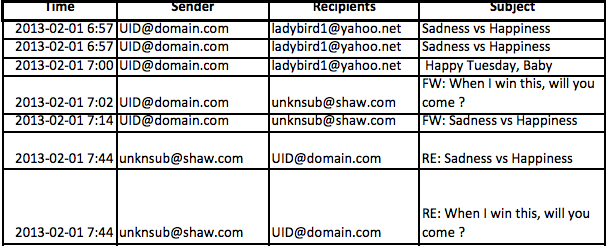
\includegraphics[width=\textwidth]{emails}
	\caption{Emails filtered by the subject line}	
\end{figure}

When looking through these emails we are looking to find any suspicious activity that might explain the attack on UID's account, or, in this case, emails sent back to UID from another source. 

The interesting information in Fig~\ref{fig:emails} is that two emails were forwarded from UID@domain.com to \textit{unknsub@shaw.com}, and then \textit{unknsub@shaw.com} responded to UID with those emails.  This explains the "returned emails" that UID had seen and reported.  

Following this, if Ulric says he didn't send those emails to \textit{unknsub@shaw.com}, then the attacker must have sent them.  There are two possibly ways this could have happened, through the corporate domain (at UID's work), or through the Outlook Web Access(OWA) gateway, which is much more likely.  Therefore, the next log that should be accessed is the IIS logs for the OWA

\bibliographystyle{IEEEtran} 
\bibliography{a5}
\end{document}